%% ----------------------------------------------------------------------
%% START OF FILE
%% ----------------------------------------------------------------------

\chapter{设计实现}
\label{cha:mainmatter}

本章介绍了论文提出的缓存系统的实现细节。从缓存系统的整体组成和架构开始,介绍缓存算法的公共接口。接下来,给出了存储卷过滤器驱动程序的实现细节,以及缓存系统是如何实现使用变长缓存块组织缓存空间。最后,给出了应用层用户配置工具提供的控制命令和对应的IOCTL代码。

\section{系统整体架构}
\label{sec:system_overview}

缓存系统的实现可分为存储卷过滤器驱动程序、缓存系统和用户配置工具几部分(图\ref{fig:sys-overview})。

\begin{figure}[H]
\centering
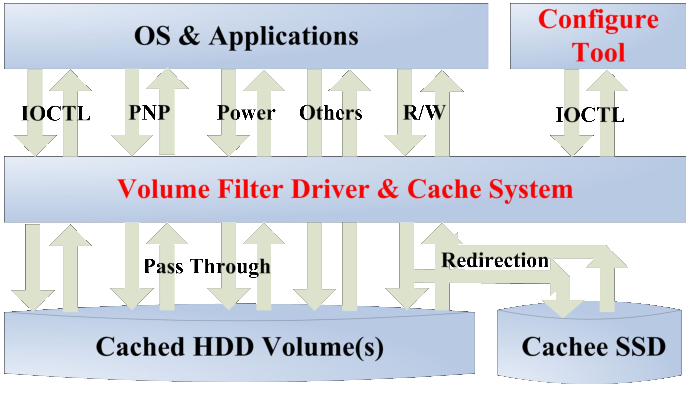
\includegraphics[width=0.6\linewidth]{./graph/sys-overview}
\caption{系统结构图}
\label{fig:sys-overview}
\end{figure}

\begin{itemize}
\item
存储卷过滤器驱动程序:过滤用户程序和操作系统对HDD卷的读写请求,供缓存算法进行SSD缓存时使用。
\item
缓存逻辑实现模块:完整的缓存系统实现,包括读写请求处理线程、缓存页替换算法、回写线程队列、缓存块索引数据结构等部分。这一模块的技术细节属于系统实现的关键技术,在上一章已经介绍。
\item
用户配置工具:提供给用户一定的缓存系统控制接口,通过IOCTL命令与驱动程序进行交互,控制过滤器驱动程序和缓存算法的运行状态。
\end{itemize}

存储卷过滤器驱动程序和缓存逻辑实现模块是系统的核心实现。这两部分虽然在逻辑上分离,但是互相依赖且存在非常多的数据交互。因此为了降低实现难度、减少模块间交互带来的性能损失,这两部分实现于同一个Windows内核模块之中(图\ref{fig:sys-flt-arch})。

\begin{figure}[H]
\centering
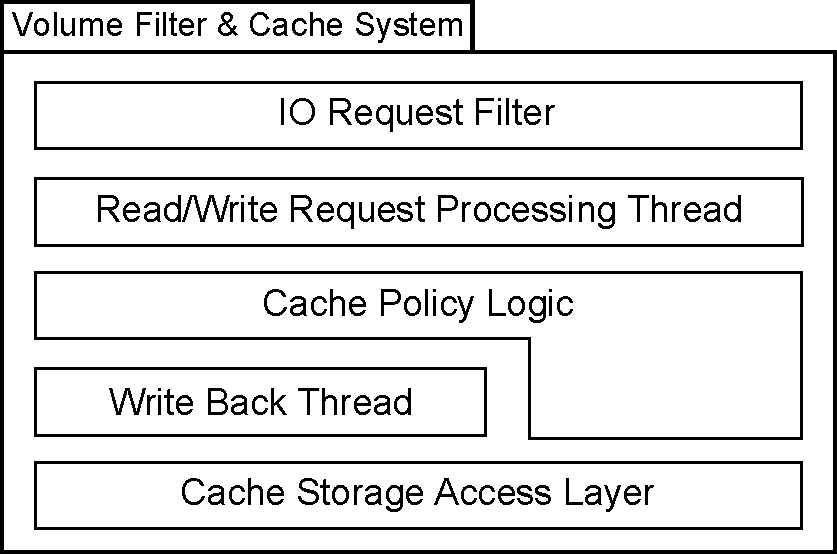
\includegraphics[width=0.6\linewidth]{./graph/sys-flt-arch}
\caption{存储卷过滤器驱动程序架构}
\label{fig:sys-flt-arch}
\end{figure}

\begin{itemize}
\item
IO请求(IRP)过滤器:过滤存储卷设备所在IO栈上的所有类型IRP,将读写类型的IRP加入读写队列;其他类型的IRP只关注存储卷上线、移除等几种特定的类型。
\item
读写请求处理线程:通过与缓存系统交互,处理加入读写队列的IO请求。
\item
缓存算法逻辑:使用SSD缓存池中的数据处理针对HDD的读写请求;利用从HDD得到的数据,结合缓存页面替换算法,更新SSD缓存池。
\item
回写线程:实现了写回(Write Back)和写穿(Write Through)两种回写策略,定期将缓存池中未同步的脏数据写回到HDD。
\item
缓存介质访问层:管理作为缓存的SSD存储卷的空间分配和读写相关操作。
\end{itemize}

%% ----------------------------------------------------------------------

\section{缓存算法通用接口}
\label{sec:cache_interface}

缓存系统实现中包含了LRU、LFU和论文提出的三种缓存页面替换算法。无论哪种页面替换算法所要完成的工作以及提供给过滤器驱动程序的接口都是一致的。为了减少系统实现中的冗余代码,论文实现过程中将缓存算法的通用接口进行了抽象,每种替换算法只要按照通用接口进行实现,系统代码就可以通过C语言宏开关的方式方便切换缓存替换算法。

通用接口分为内部和外部两类接口函数。外部接口将会被暴露给过滤器驱动程序,完成缓存系统的功能;外部函数接口的实现代码中会调用内部函数接口,虽然不同替换算法的替换策略不同,但实现中页面替换的逻辑流程仍然是相同的,因此可以为不同的算法抽象出相同的内部函数接口,减少冗余代码、方便缓存系统进行缓存替换算法间的切换。

\subsection{数据结构}

缓存系统用到了两种结构体:缓存块结构体用于映射主存块和缓存块,缓存池结构体用于组织管理缓存存储空间。

\begin{itemize}

\item 缓存块(CACHE\_BLOCK)
\\映射SSD缓存块和HDD主存块,代表了最小的缓存存储单元。
\begin{lstlisting}
typedef struct _CACHE_BLOCK
{
    ULONGLONG Index;
    ULONGLONG StorageIndex;
    BOOLEAN   Modified;
}CACHE_BLOCK, *PCACHE_BLOCK;
\end{lstlisting}
Index是HDD主存块的索引,标记了缓存块所对应的主存块在HDD中的位置。StorageIndex是SSD缓存块的索引,记录了该缓存块在缓存空间中的位置。Modified是更改标志:当回写策略是写回(Write Back)时,标记当前缓存块是否与主存同步,TRUE表示不同步需要回写,FALSE表示同步;回写策略是写穿(Write Through)时,更改标志没有意义。

\item 缓存池(CACHE\_POOL)
\\SSD缓存空间的存储块池,用于组织缓存存储块,记录缓存池的使用情况和统计信息。
\begin{lstlisting}
typedef struct _CACHE_POOL
{
    ULONG        Size;
    ULONG        Used;
    STORAGE_POOL Storage;
    ULONG32      ReadCount;
    ULONG32      WriteCount;
    ULONG32      ReadHit;
    ULONG32      WriteHit;
}CACHE_POOL, *PCACHE_POOL;
\end{lstlisting}
Size记录了缓存池内所包含的存储块总数,即缓存池的总空间大小。Used记录了缓存池内已使用存储块数量。Storage代表组织所有缓存存储空间的存储池,负责管理底层存储介质访问。ReadCount记录被缓存设备接收的读请求总数。WriteCount记录被缓存设备接收的写请求总数。ReadHit记录缓存的读请求命中总数。WriteHit记录缓存的写请求命中总数。

\end{itemize}

\subsection{外部函数接口}

外部函数接口被暴露给过滤器驱动程序,实现缓存系统的功能。

\begin{itemize}

\item InitCachePool
\\初始化缓存存储块池结构体,申请存储池空间。
\begin{lstlisting}
bool InitCachePool (
    PCACHE_POOL CachePool
);
\end{lstlisting}
传入缓存池结构体指针。初始化成功返回TRUE,否则返回FALSE。

\item DestroyCachePool
\\销毁缓存存储块池,释放存储空间。
\begin{lstlisting}
void DestroyCachePool (
    PCACHE_POOL CachePool
);
\end{lstlisting}

\item QueryAndCopyFromCachePool
\\查询缓存池中的数据是否命中偏移为Offset,长度为Length的主存储设备读请求。
\begin{lstlisting}
bool QueryAndCopyFromCachePool (
    PCACHE_POOL CachePool,
    PUCHAR Buffer,
    LONGLONG Offset,
    ULONG Length
);
\end{lstlisting}
传入缓存池结构体指针,数据位置和数据指针。如果完全命中,拷贝数据到Buffer,返回TRUE;如果不命中,返回FALSE。

\item QueryAndWriteToCachePool
\\查询缓存池中的数据是否命中偏移为Offset,长度为Length的主存储设备写请求。
\begin{lstlisting}
bool QueryAndWriteToCachePool (
    PCACHE_POOL CachePool,
    PUCHAR Buffer,
    LONGLONG Offset,
    ULONG Length
);
\end{lstlisting}
传入缓存池结构体指针,数据位置和数据指针。如果完全命中,使用Buffer中的数据更新缓存池中的数据,返回TRUE;如果不命中,返回FALSE。

\item ReadUpdataCachePool
\\使用缓存页面替换算法,利用从HDD读出的数据更新缓存池。
\begin{lstlisting}
void ReadUpdataCachePool (
    PCACHE_POOL CachePool,
    PUCHAR Buffer,
    LONGLONG Offset,
    ULONG Length
);
\end{lstlisting}
传入缓存池结构体指针,数据位置和数据指针。Buffer中是从HDD读出的偏移为Offset,长度为Length的数据。如果缓存池还有空间,加入新缓存块到缓存池;否则使用缓存页面替换算法找出缓存块进行替换。

\item WriteUpdataCachePool
\\使用缓存页面替换算法,利用已经写入HDD的数据更新缓存池。
\begin{lstlisting}
void WriteUpdataCachePool (
    PCACHE_POOL CachePool,
    PUCHAR Buffer,
    LONGLONG Offset,
    ULONG Length
);
\end{lstlisting}
传入缓存池结构体指针,数据位置和数据指针。Buffer中的数据是偏移为Offset,长度为Length的最新HDD数据。为保证数据的一致性,需要更新缓存中与HDD上最新数据(偏移为Offset,长度为Length)有重叠部分的数据。

\item IsEmpty
\\判断缓存存储块池是否为空。
\begin{lstlisting}
bool IsEmpty (
    PCACHE_POOL CachePool
);
\end{lstlisting}
传入缓存池结构体指针。如果为空返回TURE;否则返回FALSE。

\item IsFull
\\判断缓存存储块池是否存在空闲缓存块。
\begin{lstlisting}
bool IsFull (
    PCACHE_POOL CachePool
);
\end{lstlisting}
传入缓存池结构体指针。如果已满返回TURE;否则返回FALSE。

\end{itemize}

\subsection{内部函数接口}

内部函数接口在外部接口函数的实现代码中被调用。虽然不同缓存算法的替换策略不同,但总体逻辑流程相同,因此可为不同的算法抽象出相同的内部函数接口,方便在缓存替换算法之间切换。

\begin{itemize}

\item \_QueryPoolByIndex
\\查询缓存存储块池中是否存在HDD数据索引为Index的缓存块。
\begin{lstlisting}
bool _QueryPoolByIndex (
    PCACHE_POOL CachePool,
    LONGLONG Index,
    PCACHE_BLOCK *ppBlock
);
\end{lstlisting}
传入缓存池结构体指针和HDD数据块索引。如果存在,返回该缓存块的指针到ppBlock,返回TRUE;否则返回FALSE。

\item \_\_GetFreeBlock
\\从缓存存储块池中获取一个未使用的缓存块。
\begin{lstlisting}
PCACHE_BLOCK __GetFreeBlock (
    PCACHE_POOL CachePool
);
\end{lstlisting}
传入缓存池结构体指针。如果成功获取返回指向空闲缓存块的指针,从缓存池空闲缓存块计数减1;否则返回NULL。

\item \_AddNewBlockToPool
\\加入新的缓存块到缓存池中。
\begin{lstlisting}
PCACHE_BLOCK _AddNewBlockToPool (
    PCACHE_POOL CachePool,
    LONGLONG Index,
    PVOID Data,
    BOOLEAN Modified
);
\end{lstlisting}
传入缓存池结构体指针,新缓存块数据及对应的HDD索引。当存储池存在空闲空间时,加入索引为Index,数据为Data的缓存块。Modified标记传入的数据是读类型还是写类型,使用写回策略时包含写类型数据的缓存块需要被加入回写队列。如果成功加入缓存池返回新创建的缓存块指针;否则返回NULL。

\item \_FindBlockToReplace
\\从不存在空闲空间的缓存池中找出一个可替换的缓存块。
\begin{lstlisting}
PCACHE_BLOCK _FindBlockToReplace (
    PCACHE_POOL CachePool,
    LONGLONG Index,
    PVOID Data,
    BOOLEAN Modified
);
\end{lstlisting}
传入缓存池结构体指针,新缓存块数据及对应的HDD索引。当缓存块存储池满时,利用缓存页面替换算法从缓存池中选取出一个可替换的块进行替换。Modified标记传入的数据是读类型还是写类型。如果成功获取返回数据被替换的缓存块指针;否则返回NULL。

\item \_IncreaseBlockReference
\\增加缓存块的访问计数。
\begin{lstlisting}
VOID _IncreaseBlockReference (
    PCACHE_POOL CachePool,
    PCACHE_BLOCK pBlock
);
\end{lstlisting}
传入缓存池结构体指针和缓存块指针。当某个缓存块被访问时(读/写),告知告知缓存页面替换算法其访问计数增加1,以进行替换算法内部数据结构的更新。

\end{itemize}

%% ----------------------------------------------------------------------

\section{IO操作捕获函数逻辑}
\label{sec:capture_io_logic}

驱动程序通过重载卷过滤器驱动程序的分发函数达到捕获应用程序IO操作的目的。

\subsection{默认分发函数}

默认分发函数用于实现我们不需要使用的分发函数接口。对于本驱动不关心的IRP,仍需传递给底层的驱动程序才能保证程序的正常运行。
一个驱动程序可以为每个分发函数接口实现一个独立的分发函数。同样的,也可以用一个分发函数实现多种分发函数接口。默认分发函数就是一种被用来实现多种分发函数接口的函数。该函数直接跳过IO栈上当前驱动设备对象所处的位置,将IRP发送给更底层的驱动设备对象(图\ref{fig:df-default})。

\begin{figure}[H]
\centering
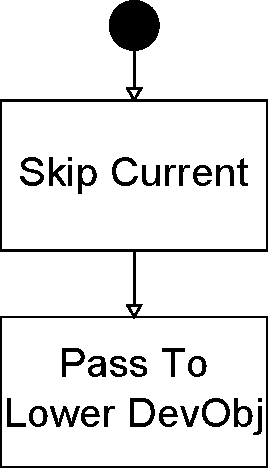
\includegraphics[width=0.2\linewidth]{./graph/df-default}
\caption{默认分发函数}
\label{fig:df-default}
\end{figure}

\subsection{电源事件分发函数}

电源事件分发函数实现了IRP\_MJ\_POWER分发函数接口。电源事件IRP包含了操作系统对硬件设备的电源操作,或是将硬件设备的电源的状态反馈给操作系统。
Windows操作系统允许传递SystemPowerState和DevicePowerState两种类型的电源状态信息。
本论文实现的存储卷过滤器驱动程序只关注SystemPowerState的PowerSystemShutdown电源事件。如图\ref{fig:df-power}所示,当包含系统即将关机信息的IRP被捕获后,电源事件分发函数会同步所有脏缓存块到HDD,并将IRP传递给更底层的设备对象;否则,跳过当前驱动设备对象,传递IRP给更底层的驱动设备对象。

\begin{figure}[H]
\centering
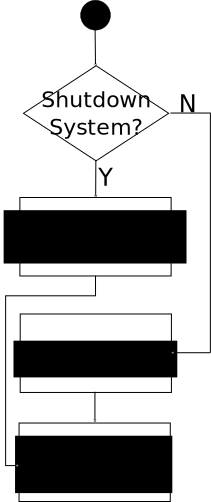
\includegraphics[width=0.3\linewidth]{./graph/df-power}
\caption{电源事件分发函数}
\label{fig:df-power}
\end{figure}

\subsection{IOCTL分发函数}

IOCTL分发函数实现了IRP\_MJ\_DEVICE\_CONTROL函数接口。IOCTL命令由Windows操作系统的IO管理器或是其他的内核驱动程序发送。大多数情况下,IOCTL类型的IRP是由用户层应用程序调用微软的Win32 API函数DeviceIoControl触发IO管理器产生的。
每当有存储卷初始化完毕将要上线时,IO管理器会给存储卷所在IO栈上的所有设备对象发送IRP\_MN\_QUERY\_REMOVE\_DEVICE的IOCTL命令。论文实现的存储卷过滤器驱动程序在过滤到此类型的IRP后,会向更底层的设备对象同步发送此IRP。确认存储卷已经上线后,检测上线的存储卷是否是目标卷。如果是目标卷,则查询目标卷的相关信息并进行相应的初始化操作,完成IRP请求;否则直接完成IRP请求(图\ref{fig:df-ioctl})。

\begin{figure}[H]
\centering
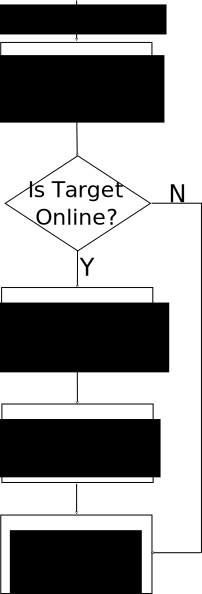
\includegraphics[width=0.25\linewidth]{./graph/df-ioctl}
\caption{IOCTL分发函数}
\label{fig:df-ioctl}
\end{figure}

\subsection{PnP事件分发函数}

PnP事件分发函数实现了IRP\_MJ\_PNP函数接口。PnP(Plug and Play)是总线在检测到硬件设备连接状态改变后,向总线驱动程序发送的一种总线信号。这种总线信号在被PnP事件管理器转换为相应类型的IRP后,会被发送给设备所在IO栈上的设备对象。
当存储卷即将被移除时,PnP事件管理器会给存储卷所在IO栈上的所有设备对象发送包含IRP\_MN\_REMOVE\_DEVICE信息的IRP。论文实现的存储卷过滤器驱动程序在过滤到此类型的IRP后,会向更底层的设备对象同步发送此IRP。确认存储卷被移除后,如果是被SSD缓存的卷,则停止工作线程、释放缓存索引占用的内存空间、从底层设备对象分离并移除当前驱动程序的设备对象,最终完成IRP请求(图\ref{fig:df-pnp})。

\begin{figure}[H]
\centering
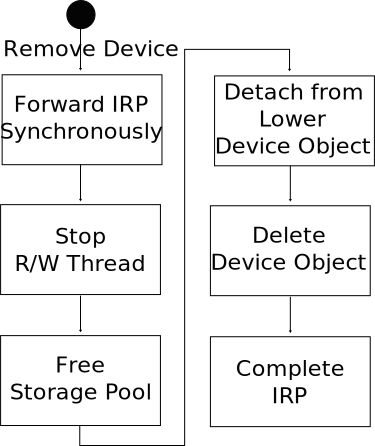
\includegraphics[width=0.45\linewidth]{./graph/df-pnp}
\caption{PnP事件分发函数}
\label{fig:df-pnp}
\end{figure}

\subsection{读写分发函数}

存储卷的所有读和写操作都是通过IRP\_MJ\_READ和IRP\_MJ\_WRITE函数接口的实现函数完成的。论文实现的存储卷过滤器驱动程序使用一个读写分发函数统一实现了这两种函数接口。
该函数不会立即对包含读写请求的IRP进行处理(图\ref{fig:df-rw}),而是将IRP加入到驱动程序的读写请求队列中供驱动程序创建的读写线程处理,并返回IRP正在处理中的状态。

\begin{figure}[H]
\centering
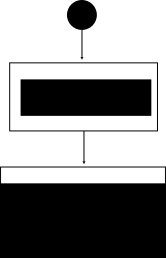
\includegraphics[width=0.2\linewidth]{./graph/df-rw}
\caption{读写分发函数}
\label{fig:df-rw}
\end{figure}

读写线程检测到读写队列不为空时,从队列头部依次处理每个读写请求(图\ref{fig:df-rw-thread})。这样做的好处是可以使并行的读写操作串行化,避免了可能的数据访问冲突,同时还可以减少锁操作对性能的消耗。

\begin{figure}[H]
\centering
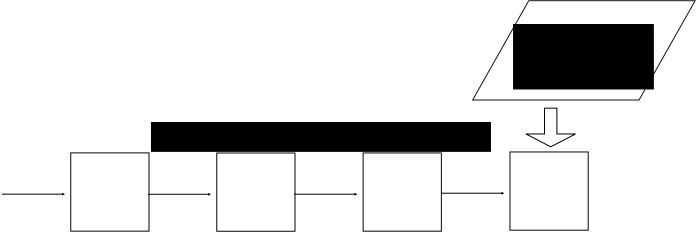
\includegraphics[width=0.5\linewidth]{./graph/df-rw-thread}
\caption{读写处理内核线程}
\label{fig:df-rw-thread}
\end{figure}

读写线程中对读和写请求的处理逻辑相似但细节不同。图\ref{fig:df-proc-read}展现了读请求的处理逻辑。

\begin{figure}[H]
\centering
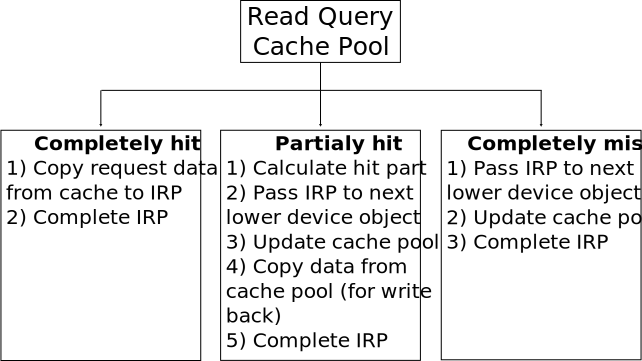
\includegraphics[width=0.75\linewidth]{./graph/df-proc-read}
\caption{读写线程读请求处理逻辑}
\label{fig:df-proc-read}
\end{figure}

图\ref{fig:df-proc-write}展现了写请求的处理逻辑。写请求和读请求的处理都存在更新SSD缓存池的操作,但实现的细节并不相同:读请求直接使用读请求获得的HDD数据更新SSD;写请求依据回写策略的不同又可分为写穿(Write Through)和写回(Write Back)两类。写穿策略会先将写请求的数据应用于HDD,再去更新SSD。写回策略直接使用写请求的数据更新SSD,回写线程负责将缓存中的脏数据同步回HDD。这两种回写策略在\ref{sec:wb_strategy}节被详细描述。

\begin{figure}[H]
\centering
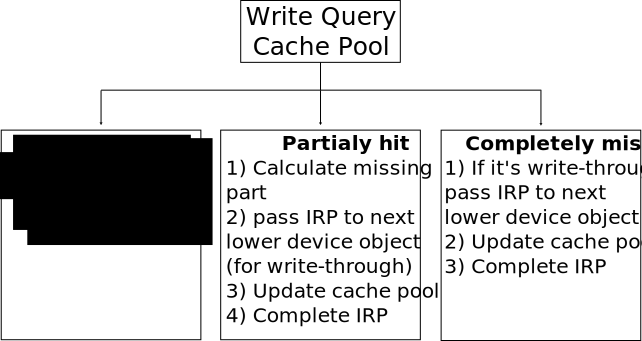
\includegraphics[width=0.75\linewidth]{./graph/df-proc-write}
\caption{读写线程写请求处理逻辑}
\label{fig:df-proc-write}
\end{figure}

%% ----------------------------------------------------------------------

\section{可变长缓存块的处理}

硬盘的最小存储单元是扇区,大小为512字节,因此Windows的IO管理器产生的读写请求会以512字节对齐。缓存系统中,缓存空间和主存储空间一般也会以512字节的大小进行划分。

应用程序产生的磁盘读写操作请求的大小可能会达到几兆字节,对于这种请求,需要以512字节进行分段,多次查询缓存池,对系统性能的影响较大。为了提升缓存系统性能,本论文实现了缓存块大小的可变长度机制:读写请求由IO管理器产生,512字节大小对齐无法改变;缓存空间使用512字节的倍数大小进行划分。这么做对于较大的读写请求,一方面可以减少分段的个数,降低多次查询缓存池对性能的影响;另一方面从缓存池内向外拷贝数据时,每次拷贝的数据量变大,拷贝效率更高。

但是,由于读写请求的大小和缓存空间的划分不是以相同字节数目对齐,这就需要在查询缓存池和拷贝缓存数据时解决读写请求不对齐的问题。如图\ref{fig:vsize-cache-block}所示,不对齐部分只可能出现在读写请求的开头(f\_broken)和结尾(e\_broken)部分,只要对这部分数据进行特殊处理,其余部分按对齐方式正常处理即可。

\begin{figure}[H]
\centering
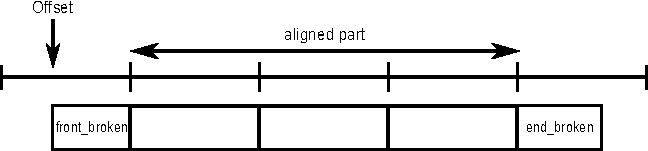
\includegraphics[width=0.75\linewidth]{./graph/vsize-cache-block}
\caption{读写大小和缓存划分不对齐的情况}
\label{fig:vsize-cache-block}
\end{figure}

下面分别给出了读、写请求不对齐时缓存命中与不命中情况的处理方式:

\begin{itemize}

\item 读请求命中的处理
\begin{enumerate}
\item 检查对齐部分所属的数据块是否在缓存池中缓存。
\item 检查f\_broken和e\_broken部分的所属的数据块是否在缓存池中缓存。
\item 如果完全命中,在从缓存池中拷贝数据时,需要注意f\_broken和e\_broken部分拷贝数据时的偏移和长度。
\end{enumerate}

\item 读请求未命中的处理
\begin{enumerate}
\item 向下发送读请求,获得主存数据。
\item 只使用对齐部分所属的数据块更新缓存池。
\end{enumerate}

\item 写请求命中的处理
\begin{enumerate}
\item 检查对齐部分所属的数据块是否在缓存池中缓存。
\item 检查f\_broken和e\_broken部分的所属的数据块是否在缓存池中缓存。
\item 如果完全命中,在向缓存池中写入数据时,需要注意在写入f\_broken和e\_broken部分数据时的偏移和长度。
\end{enumerate}

\item 写请求未命中的处理
\begin{enumerate}
\item 使用对齐部分所属的命中数据块更新缓存池。
\item 检查f\_broken和e\_broken部分的所属的数据块命中。如果命中,写入并注意f\_broken和e\_broken部分写入数据时的偏移和长度;未命中,当回写策略是写回(Write Back)模式时,由于f\_broken和e\_broken部分的数据无法构成完整的缓存数据块,故而需要将这两部分数据直接写入主存储器。
\end{enumerate}

\end{itemize}

%% ----------------------------------------------------------------------

\section{用户配置工具}
\label{sec:config_utility}

系统提供了命令行的用户配置工具,在用户层和内核层的驱动程序进行交互。通过驱动设备对象提供的IOCTL命令,来完成两个方面的功能:
\begin{enumerate}
\item 配置缓存系统的运行状态。包括启动、停止和设置作为缓存的卷。
\item 获得缓存系统的统计数据。获得IO统计信息,如读写次数和命中率。
\end{enumerate}

配置工具启动后,依据用户输入的命令完成相应操作。工具提供如下几种种命令:

\begin{itemize}
\item start
\\描述:为某个指定的HDD存储卷开启SSD缓存。
\\使用:start  [disk\_number]  [volume\_number]
\\IOCTL:IOCTL\_DF\_START

\item stop
\\描述:停止某个HDD存储卷上的SSD缓存。
\\使用:stop  [disk\_number]  [volume\_number]
\\IOCTL:IOCTL\_DF\_STOP

\item stat
\\描述:获取某个存储卷的统计数据。包括读、写操作次数,缓存命中率以及使用情况。
\\使用:stat  [disk\_number]  [volume\_number]
\\IOCTL:IOCTL\_DF\_GET\_STAT

\item clear
\\描述:清除某个存储卷的统计数据。
\\使用:clear  [disk\_number]  [volume\_number]
\\IOCTL:IOCTL\_DF\_CLEAR\_STAT

\item quite
\\描述:设置驱动程序不向内核日志输出任何日志信息。
\\使用:quite
\\IOCTL:IOCTL\_DF\_QUIET

\item verbose
\\描述:开启驱动程序的向内核日志的所有日志信息输出。
\\使用:verbose
\\IOCTL:IOCTL\_DF\_VERBOSE

\item verify
\\描述:开启或关闭SSD缓存池内数据和HDD数据的一致性验证,默认是关闭的,开启对性能影响明显,只做调试使用。
\\使用:verify
\\IOCTL:IOCTL\_DF\_VERIFY

\item q
\\描述:退出用户配置工具。
\\使用:q
\end{itemize}

%% ----------------------------------------------------------------------
%%% END OF FILE
%% ----------------------------------------------------------------------